\begin{problem}[Hatcher {\S}2.1, Ex.\@ 17]
\begin{enumerate}[label=(\alph*)]
\item Compute the homology groups $H_n(X,A)$ when $X$ is $S^2$ or
  $S^1\times S^1$ and $A$ is a finite set of points in $X$.
\item Compute the groups $H_n(X,A)$ and $H_n(X,B)$ for $X$ a closed
  orientable surface of genus two with $A$ and $B$ the circles shown. [What
  are $X/A$ and $X/B$?]
\end{enumerate}
\end{problem}
\begin{proof}
\textbf{(a)} As a consequence of 2.16, we have a long exact sequence on relative
homology
\begin{equation}
\label{eq:long-exact-sequence-on-relative-hom}
\cdots\longrightarrow
H_n(A)\longrightarrow
H_n(X)\longrightarrow
H_n(X,A)\longrightarrow
H_{n-1}(A)\longrightarrow
\cdots.
\end{equation}
Now, specifying $X$ to be $S^2$, we know, by 2.8, 2.6 and 2.14, that
$H_n(A)\cong 0$ for all $n>0$ and $H_0(A)\cong \bigoplus_{|A|}\bfZ$, and
$H_n(S^2)\cong 0$ for $n\neq 2,0$ and $H_n(S^2)\cong\bfZ$ otherwise. Hence,
the long exact sequence (\ref{eq:long-exact-sequence-on-relative-hom})
turns into
\begin{equation}
\label{eq:long-exact-sequence}
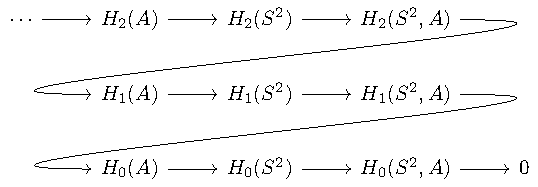
\includegraphics{hw-3-long-exact-sequence-1}
\end{equation}
which, filling in our computed values for $H_n(A)$ and $H_n(S^2)$, further
becomes
\begin{equation}
\label{eq:long-exact-sequence-of-s-2}
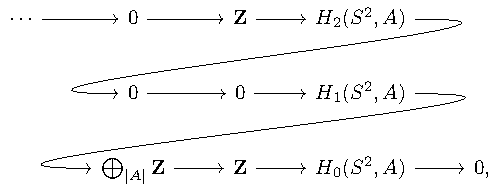
\includegraphics{hw-3-long-exact-sequence-s-2}
\end{equation}
with all other $n>2$ homology groups for $A$ and $S^2$ being $0$. That last
remark immediately tells us that, by exactness, $H_n(S^2,A)=0$ for all
$n>2$. Starting from the bottom of \eqref{eq:long-exact-sequence-of-s-2},
exactness at $H_2(S^2,A)$ tells us that $H_2(S^2,A)\cong\bfZ$ since the
zero maps to the left and right
\[
\cdots\longrightarrow 0\longrightarrow \bfZ\longrightarrow H_2(S^2,A)\longrightarrow 0\longrightarrow\cdots
\]
tells us that the map $\bfZ\to H_2(S^2,A)$ is an isomorphism. If we look at
the reduced homology, the bottom row of
\eqref{eq:long-exact-sequence-of-s-2} becomes
\[
\cdots\longrightarrow
0\longrightarrow
\widetilde H_1(S^2,A)\longrightarrow
\bigoplus_{|A|-1}\bfZ\longrightarrow
0\longrightarrow\widetilde H_0(S^2,A)
\longrightarrow 0.
\]
By exactness at $\widetilde H_1(S^2,A)$, we have $H_1(S^2,A)\cong\widetilde
H_1(S^2,A)\cong\bigoplus_{|A|-1}\bfZ$ and, last but not least, exactness at
$\widetilde H_0(S^2,A)\cong 0$ gives us $H_0(S^2,A)\cong\bfZ$. In summary,
we have
\begin{equation}
  \label{eq:homology-of-s-2-a}
H_n(S^2,A)=
\begin{cases}
\bfZ&\text{if $n=0,2$}\\
\bigoplus_{|A|-1}\bfZ&\text{if $n=1$}\\
0&\text{otherwise}
\end{cases}.
\end{equation}
\\\\
\textbf{(b)} From 2.27 we know that
$H_n^\Delta(S^1\times S^1)\cong H_n(S^1\times S^1)$ so from 2.3, we know
that the homology of the torus $S^1\times S^1$ is
\begin{equation}
\label{eq:homology-of-s-1-s-1}
H_n(S^1\times S^1)=
\begin{cases}
\bfZ\oplus\bfZ&\text{if $n=1$}\\
\bfZ&\text{if $n=2,0$}\\
0&\text{otherwise}
\end{cases}.
\end{equation}
Skipping directly, to our calculation, we have the long exact sequence
\begin{equation}
  \label{eq:long-exact-sequence-s-1-s-1}
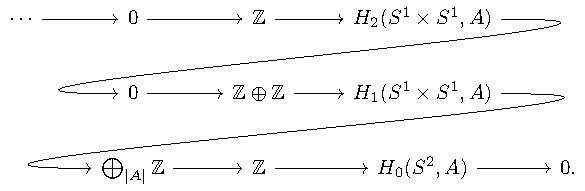
\includegraphics{hw-3-long-exact-sequence-s-1-s-1}
\end{equation}
It is clear from exactness that $H_2(S^1\times S^1,A)\cong\bfZ$ and
$H_0(S^1\times S^1,A)\cong\bfZ$. What is not clear is what $H_1(S^1\times
S^1,A)$ is. Exactness at $\bfZ\oplus\bfZ$ tells us that
$\bfZ\oplus\bfZ\hookrightarrow H_1(S^1\times S^1,A)$ and, looking at the
reduced homology, exactness at $\bigoplus_{|A|-1}\bfZ$ tells us that
$H_1(S^1\times S^1,A)\twoheadrightarrow\bigoplus_{|A|-1}\bfZ$. Thus,
we have $\bigoplus_{|A|-1}\bfZ\cong H_1(S^1\times S^1,A)/\bfZ\oplus\bfZ$
from which we can deduce that $H_1(S^1\times
S^1,A)\cong\bigoplus_{|A|+1}\bfZ$.\footnote{I know this is not strictly
  correct, but the approach I took to solve the problem required me to
  construct an inverse map $H_1(S^1\times
  S^1,A)\leftarrow\bigoplus_{|A|-1}\bfZ$, but this is difficult.} In summary, the relative homology of
$S^1\times S^1$ with respect to $A$ is
\begin{equation}
  \label{eq:homology-of-s-1-s-1-a}
H_n(S^1\times S^1,A)=
\begin{cases}
\bfZ&\text{if $n=2,0$}\\
\bigoplus_{|A|+1}\bfZ&\text{ if $n=1$}\\
0&\text{otherwise}
\end{cases}.
\end{equation}
\qedhere
\end{proof}
\newpage

\begin{problem}[Hatcher {\S}2.2, Ex.\@ 1]
Prove the Brouwer fixed point theorem for maps $f\colon D^n\to D^n$ by
applying degree theory to the map $S^n\to S^n$ that sends both the northern
and southern hemispheres of $S^n$ to the southern hemisphere via $f$. [This
was Brouwer’s original proof.]
\end{problem}
\begin{proof}
Seeking a contradiction, suppose $f\colon D^n\to D^n$ has no fixed
point. Let $N$ and $S$ denote, respectively, the northern and southern
hemisphere meeting at the equator of $S^n$. Now, since the disk $D^n\approx
S$, we may as well identify $D^n$ with $S$ and consider the map $f\colon
D^n\to D^n$ as the map $S\to S$ by composing with the homeomorphism. Define
a map $g\colon S^n\to S^n$ by
\begin{equation}
\label{eq:half-antipodal-map}
g
\coloneqq
\begin{cases}
r&\text{on $N$}\\
\Id&\text{on $S$}
\end{cases}.
\end{equation}
Note that the map $g$ is continuous by the pasting lemma since
$g\restriction_S=\Id$ and $g\restriction_N=r$ are continuous and $r$ fixes
points at the equator $N\cap S$. Now, consider the map $F\colon S^n\to S^n$
given by the composition $\iota\circ f\circ g$ where $\iota\colon
S\hookrightarrow S^n$ is the inclusion $S\subset S^n$. This map has no
fixed points since $f$ has no fixed point hence, by property (g) of the
degree, $\deg F=(-1)^{n+1}$. But $F$ is not onto, therefore $\deg
F=0$. This is a contradiction.
\end{proof}
\newpage

\begin{problem}[Hatcher {\S}2.2, Ex.\@ 6]
Show that every map $S^n\to S^n$ can be homotoped to have a fixed point
if $n>0$.
\end{problem}
\begin{proof}
The result follows from 4.25 since a map $f\colon S^n\to S^n$ without any
fixed points is homotopic to the antipodal map. Since the antipodal map has
degree $-1$ or $1$ depending on $n$, it follows that the antipodal map is
homotopic to either the identity map or a reflection map, both of which
have fixed points.
\end{proof}
\newpage

\begin{problem}
Let $\calU$ be an open cover of $X$. Prove that the inclusion of
$C_*^{\calU}(C)$ into $C_*(X)$ is a chain homotopy equivalence.
\end{problem}
\begin{proof}
This is proposition 2.21 in the book. I will summarize the proof in four
steps here.
\begin{enumerate}[label=\textbf{(\arabic*)}]
\item (Barycentric subdivision) Given a simplex $[v_0,...,v_n]$ its
  barycenter is the point $b=\sum_it_iv_i$ whose barycentric coordinates
  $t_i$ are all equal, i.e., $t_i=1/(n+1)$ for all $i$. The barycentric
  subdivision of $\left[v_0,...,v_n\right]$ is the decomposition of
  $[v_0,...,v_n]$ into the $n$-simplices $\left[b,w_0,...,w_{n-1}\right]$,
  where

\item
\item
\item
\end{enumerate}
\end{proof}

%%% Local Variables:
%%% mode: latex
%%% TeX-master: "../MA572-HW-Current"
%%% End:
